\documentclass[11pt]{article}

% Shared preamble for main.tex and supplementary.tex.
% --- page and typography ---
\usepackage[a4paper,margin=1in]{geometry}
\usepackage{microtype}
\usepackage[T1]{fontenc}
\usepackage{lmodern}
\linespread{1.05}

% --- math, units, figures, tables ---
\usepackage{amsmath}
\usepackage{siunitx}
\sisetup{detect-all, range-phrase={\text{--}}, range-units=single}
\usepackage{graphicx}
\graphicspath{{figures/}{../figures/}}
\usepackage{booktabs}
\usepackage[font=small,labelfont=bf]{caption}
\usepackage{placeins}

% --- references ---
\usepackage[backend=biber,style=numeric-comp,sorting=none,giveninits=true,maxbibnames=8,doi=true,url=false,isbn=false]{biblatex}
\addbibresource{references.bib}

% --- links and cross-refs (xr-hyper before hyperref, cleveref last) ---
\usepackage{xr-hyper}
\usepackage[hidelinks]{hyperref}
\usepackage[capitalise,nameinlink]{cleveref}

% Scrub PDF document properties so metadata stays anonymous for the EJP
% double-anonymous build (harmless in the named build).
\hypersetup{pdfauthor={},pdfsubject={},pdfkeywords={}}

% Reusable notation. Keep small; do not over-abstract.
\newcommand{\LD}{\textit{L/D}}
\newcommand{\ms}{\,\unit{\meter\per\second}}
\newcommand{\degr}{^{\circ}}
\newcommand{\cgfrac}{x_\mathrm{cg}}
\newcommand{\npfrac}{x_\mathrm{np}}

% numbers.tex: generated by analysis/export_numbers.py from metrics.json.
% Do not edit by hand; rerun the pipeline.

\newcommand{\nRelief}{10.2}
\newcommand{\nAspect}{230}
\newcommand{\nSlopeMean}{5.2}
\newcommand{\nSlopePninety}{12.8}
\newcommand{\nSlopeRadius}{400}
\newcommand{\nLiftIntoWind}{40}
\newcommand{\nLiftAlongSlope}{192}
\newcommand{\nContour}{5.1}
\newcommand{\nValleyDrop}{9.2}
\newcommand{\nHours}{175\,320}
\newcommand{\nFavPct}{15.6}
\newcommand{\nFavLo}{14.3}
\newcommand{\nFavHi}{17.0}
\newcommand{\nFavHours}{1\,370}
\newcommand{\nFavWinter}{21.1}
\newcommand{\nSWAnyPct}{34.3}
\newcommand{\nSWSixPct}{10.3}
\newcommand{\nSWSixHours}{906}
\newcommand{\nSWEightPct}{3.4}
\newcommand{\nSWEightLo}{2.9}
\newcommand{\nSWEightHi}{3.9}
\newcommand{\nSWEightHours}{296}
\newcommand{\nRidgePeak}{1.5}
\newcommand{\nRidgeWind}{8}
\newcommand{\nRidgeFormula}{1.8}
\newcommand{\nSinkBest}{1.9}
\newcommand{\nSinkNominal}{3.1}
\newcommand{\nRidgeMatchWind}{10}
\newcommand{\nTrimSpeed}{15.1}
\newcommand{\nMass}{80}
\newcommand{\nArea}{7}
\newcommand{\nCLtrim}{0.8}
\newcommand{\nTower}{18}
\newcommand{\nJump}{2}
\newcommand{\nHeightToTrim}{11.5}
\newcommand{\nLDStillSteady}{11.1}
\newcommand{\nStillRangeBest}{14}
\newcommand{\nStillRangeSteady}{142}
\newcommand{\nMaxRangeInto}{110}
\newcommand{\nMinWindBest}{5.7}
\newcommand{\nMinWindNominal}{10.6}
\newcommand{\nRangeEightBest}{271}
\newcommand{\nRangeEightNominal}{111}
\newcommand{\nRangeEightIntoBest}{104}
\newcommand{\nMinWindTowerLo}{6.6}
\newcommand{\nMinWindTowerHi}{3.8}
\newcommand{\nARlo}{3}
\newcommand{\nARhi}{5}
\newcommand{\nElo}{0.6}
\newcommand{\nEhi}{0.8}
\newcommand{\nCDzlo}{0.05}
\newcommand{\nCDzhi}{0.15}
\newcommand{\nLDlo}{3.1}
\newcommand{\nLDhi}{7.9}
\newcommand{\nLDnom}{4.7}
\newcommand{\nNPnotail}{0.25}
\newcommand{\nNPtail}{0.53}
\newcommand{\nCGlo}{0.35}
\newcommand{\nCGhi}{0.55}
\newcommand{\nCGonset}{0.30}
\newcommand{\nTloss}{0.74}
\newcommand{\nTdoubleRep}{0.24}
\newcommand{\nTdoubleFwd}{0.60}
\newcommand{\nTdoubleAft}{0.16}
\newcommand{\nTdoubleInLo}{0.12}
\newcommand{\nTdoubleInHi}{0.89}
\newcommand{\nFlightTime}{16}
\newcommand{\nReactLo}{0.15}
\newcommand{\nReactHi}{0.3}
\newcommand{\nSamples}{40\,000}
\newcommand{\nReachSlope}{6.9}
\newcommand{\nReachSlopeLo}{6.6}
\newcommand{\nReachSlopeHi}{7.1}
\newcommand{\nReachSlopeN}{2\,748}
\newcommand{\nReachInto}{0}
\newcommand{\nReachIntoHi}{0.01}
\newcommand{\nMedRangeSlope}{83}
\newcommand{\nMedRangeInto}{62}
\newcommand{\nNinetyRangeSlope}{180}
\newcommand{\nShortFifty}{34}
\newcommand{\nMedWindReach}{7.6}
\newcommand{\nTenWindReach}{5.4}
\newcommand{\nMedLDReach}{5.8}
\newcommand{\nMedLDAll}{4.7}
\newcommand{\nMedFlightReach}{24}
\newcommand{\nTdoubleMC}{0.29}
\newcommand{\nTdoubleMCpnn}{1.6}
\newcommand{\nTibiaLo}{7.5}
\newcommand{\nTibiaHi}{11.3}
\newcommand{\nOnsetMid}{9.7}
\newcommand{\nOnsetLo}{6.1}
\newcommand{\nOnsetHi}{14.1}
\newcommand{\nCtrlVzMed}{2.2}
\newcommand{\nCtrlVzMax}{4.1}
\newcommand{\nDepVzMed}{10.1}
\newcommand{\nDepAngLo}{35}
\newcommand{\nDepAngHi}{70}
\newcommand{\nVreachLo}{10.3}
\newcommand{\nVreachHi}{19.4}
\newcommand{\nPbreakDep}{58}
\newcommand{\nDecelG}{26}
\newcommand{\nExSinkNom}{3.1}
\newcommand{\nExUsoarNom}{14.2}
\newcommand{\nExSinkHi}{1.9}
\newcommand{\nExUsoarHi}{8.5}
\newcommand{\nExWilsonHalf}{0.25}
\newcommand{\nExHeadwind}{13.1}
\newcommand{\nExVdepFifty}{11.6}


\hypersetup{pdftitle={Wind, slope, and the want of a tail}}
% Table S1, Figure S1 and Supplementary S1-S4 are labelled in supplementary.tex.
\externaldocument{supplementary}


\title{\bfseries Wind, slope, and the want of a tail:\\
a computational feasibility study of Eilmer of Malmesbury's flight}

% Author block per ~/dev/Rules/AUTHORSHIP.md. EJP uses double-anonymous review;
% the named block is the default, and defining \anon (see main_anon.tex) produces
% the blind build: no author block, no acknowledgements, no repository links.
\ifdefined\anon
  \author{}
\else
  \author{David H. Silver \\[3pt]
    {\normalsize Remiza, Poughkeepsie, NY, USA} \\[1pt]
    {\small Corresponding author: \texttt{david@remiza.ai} \,\textperiodcentered\, ORCID 0000-0002-3071-304X}}
\fi
\date{}

\begin{document}
\maketitle

\begin{abstract}
\noindent
William of Malmesbury records that early in the eleventh century Eilmer, a fellow monk,
fixed wings to his hands and feet, launched from a tower, travelled ``more than a furlong''
(about \SI{\nTarget}{\meter}), and fell, breaking both legs.
He blamed the missing tail.
This paper tests the account with undergraduate mechanics (glide, slope lift, pitch
stability, impact), public terrain and wind data, and a Monte Carlo sample over the unknown
apparatus and launch day.
From a walking-pace launch a glider loses about \SI{\nHeightToTrim}{\meter} reaching its
\SI{\nTrimSpeed}{\meter\per\second} flying speed, so a long flight needs a strong wind.
Flown into that wind over the valley, none of \nSamples\ sampled cases covers
\SI{\nTarget}{\meter}.
Along the southwest-facing slope, in ridge lift, \SI{\nReachSlope}{\percent} do
(\SI{95}{\percent} confidence interval \numrange{\nReachSlopeLo}{\nReachSlopeHi}\,\%), at a
median launch wind of \SI{\nMedWindReach}{\meter\per\second}.
Without a tail a pitch disturbance doubles in a median \SI{\nTdoubleMC}{\second}, comparable
to human reaction time, in a flight of about \SI{\nMedFlightReach}{\second}; a tail removes
the divergence.
A controlled arrival does not break the legs; one after loss of pitch control often does.
The account is physically possible but marginal, and the missing tail is a sufficient cause
of the fall.
Each step is a student exercise with worked answers.
\end{abstract}

\section{Introduction}

William of Malmesbury, writing his \textit{Gesta Regum Anglorum} in about 1125, records
that Eilmer, an older monk of his own abbey, had in his youth fixed wings to his hands and
feet, launched from a tower, and travelled ``more than a furlong'' before he fell, broke both
legs, and was lame for the rest of his life \autocite{williamMalmesbury_gesta}.
Eilmer, William adds, used to say that he fell because he had forgotten to fit a tail.
Lynn White's study of the passage established it as the earliest credible account of a
gliding attempt in Western Europe \autocite{white1961eilmer}.

The short account names a launch point, a distance, a wind, a failure, an injury, and a
cause, and undergraduate physics can check each one.
Could Eilmer's flight have happened at Malmesbury, and is a missing tail enough to explain
the fall?
No source describes Eilmer's apparatus beyond its wings, so the models sample its unknown
parameters.

As a teaching case for undergraduate mechanics, the problem assumes calculus, Newtonian
mechanics, and elementary probability, and suits students from the second year onwards and
their instructors.
Answering it needs the energy balance of a glider at launch, flight in a moving air mass,
lift over a slope, the neutral-point criterion for pitch stability, the growth rate of an
unstable mode, Monte Carlo estimation with confidence intervals, and the mechanics of a
feet-first impact.
Each step uses public data and a few lines of code, gives a number to check against the
text, and becomes an exercise in \cref{sec:teaching}.

\section{The source and the site}
\label{sec:source}

William wrote a century after the flight and could have heard it from men who knew Eilmer
\autocite{white1961eilmer,thomson2004eilmer_odnb}.
Supplementary S1 gives his Latin and a standard translation.
He says Eilmer ``collected the breeze on the summit of a tower'' and that the violence
of the wind and the swirling of the air brought him down.
The traditional date is about 1000--1010.
\textcite{aitcheson2026date} argues it could be as late as the early 1040s.
Launch weather is sampled from a modern climatology, so the year does not matter.

Other early flight accounts are mostly legend \autocite{paz2013humanflight}.
The only one with a stated device is that of Abbas ibn Firnas of ninth-century Córdoba,
whom later Andalusian chronicles credit with a structure of feathers and silk and a bad
landing, also blamed on a missing tail \autocite{white1961eilmer,anderson2024bridge}.
\textcite{hallion2003takingflight} reads it as closer to a parachute descent.
Neither gives dimensions or construction.
With no historical basis for a specific design, the models sample wing area, mass, shape,
and drag over wide ranges (Supplementary \cref{tab:priors}).

\begin{figure}[htbp]
  \centering
  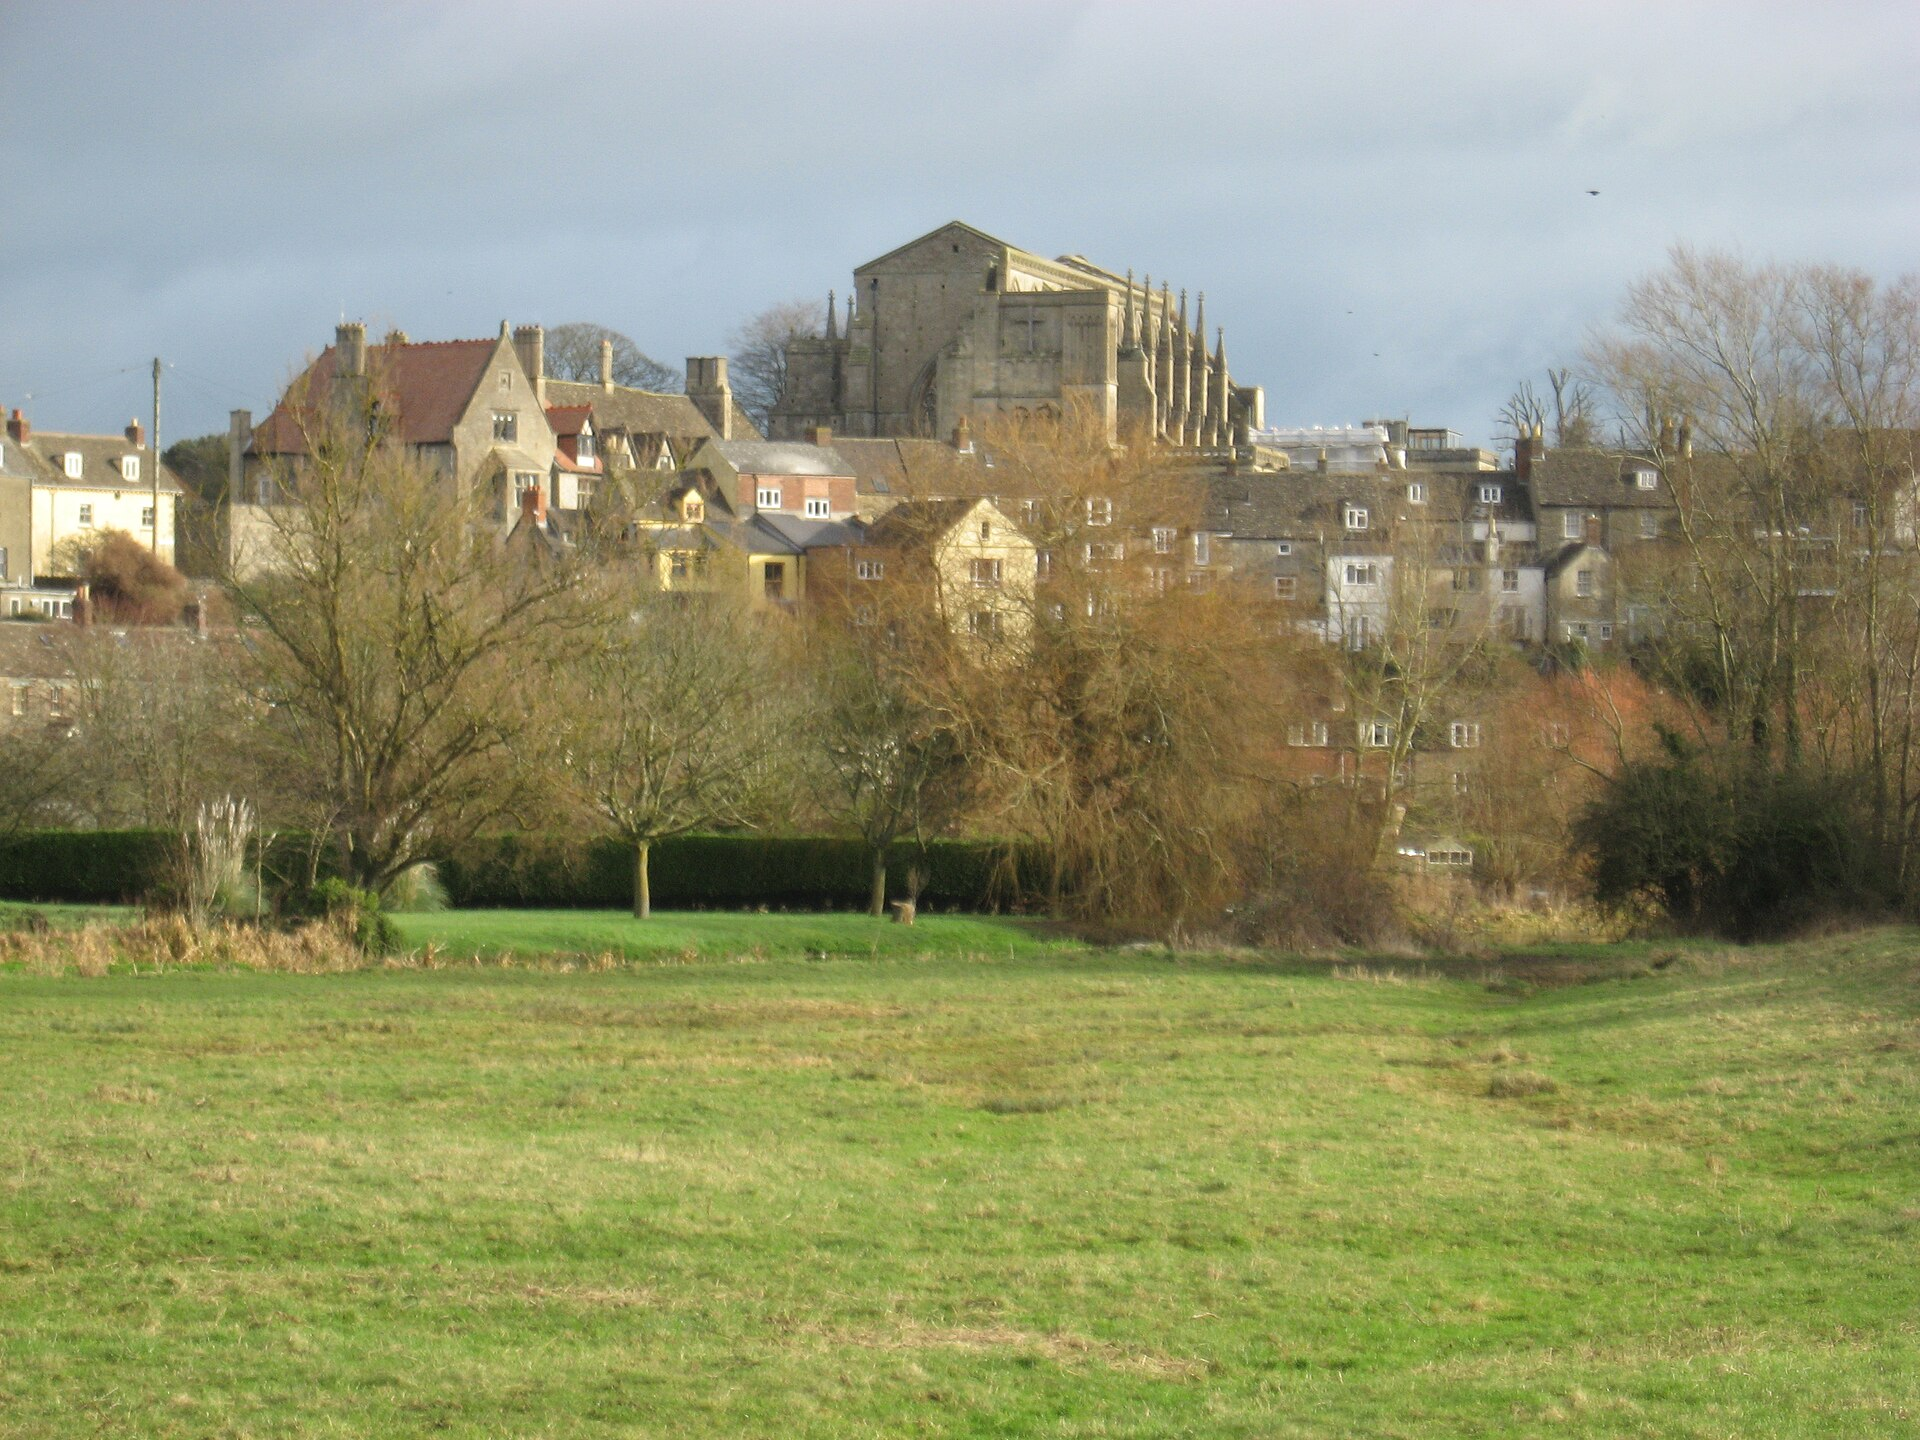
\includegraphics[width=0.8\linewidth]{fig_abbey_photo.jpg}
  \caption{\textbf{Malmesbury Abbey seen from the southwest.}
  The view looks northeast from the Avon water meadows, about \SI{300}{\meter} west-southwest
  of the abbey, up the slope the prevailing wind strikes.
  The present church is twelfth-century; Eilmer's Anglo-Saxon church and tower do not
  survive, so the launch point is taken as the abbey site and the tower height is sampled.
  Photograph: Dr Duncan Pepper (2012, Geograph and Wikimedia Commons), CC BY-SA 2.0.}
  \label{fig:photo}
\end{figure}

The abbey stands on a narrow spur between two arms of the Avon.
The sampled tower height, \SIrange{\nTowerLo}{\nTowerHi}{\meter}, brackets White's estimate of about
\SI{\nTower}{\meter} \autocite{white1961eilmer}.
\textcite{woosnam1986eilmer} puts the flight down the steep slope southwest of the abbey
towards the river, the side shown in \cref{fig:photo}.

\section{Methods}
\label{sec:methods}

\subsection{Terrain}

The terrain comes from the Amazon Web Services (AWS) Terrain Tiles, a digital elevation
model (DEM) with a grid spacing of about \SI{\nDEMres}{\meter}.
Slope and aspect (the direction a slope faces) are computed within
\SI{\nSlopeRadius}{\meter} of the abbey, along with a southwest--northeast elevation section.
The grid smooths the steep edge of the spur, so slopes are lower bounds.

\begin{figure}[htbp]
  \centering
  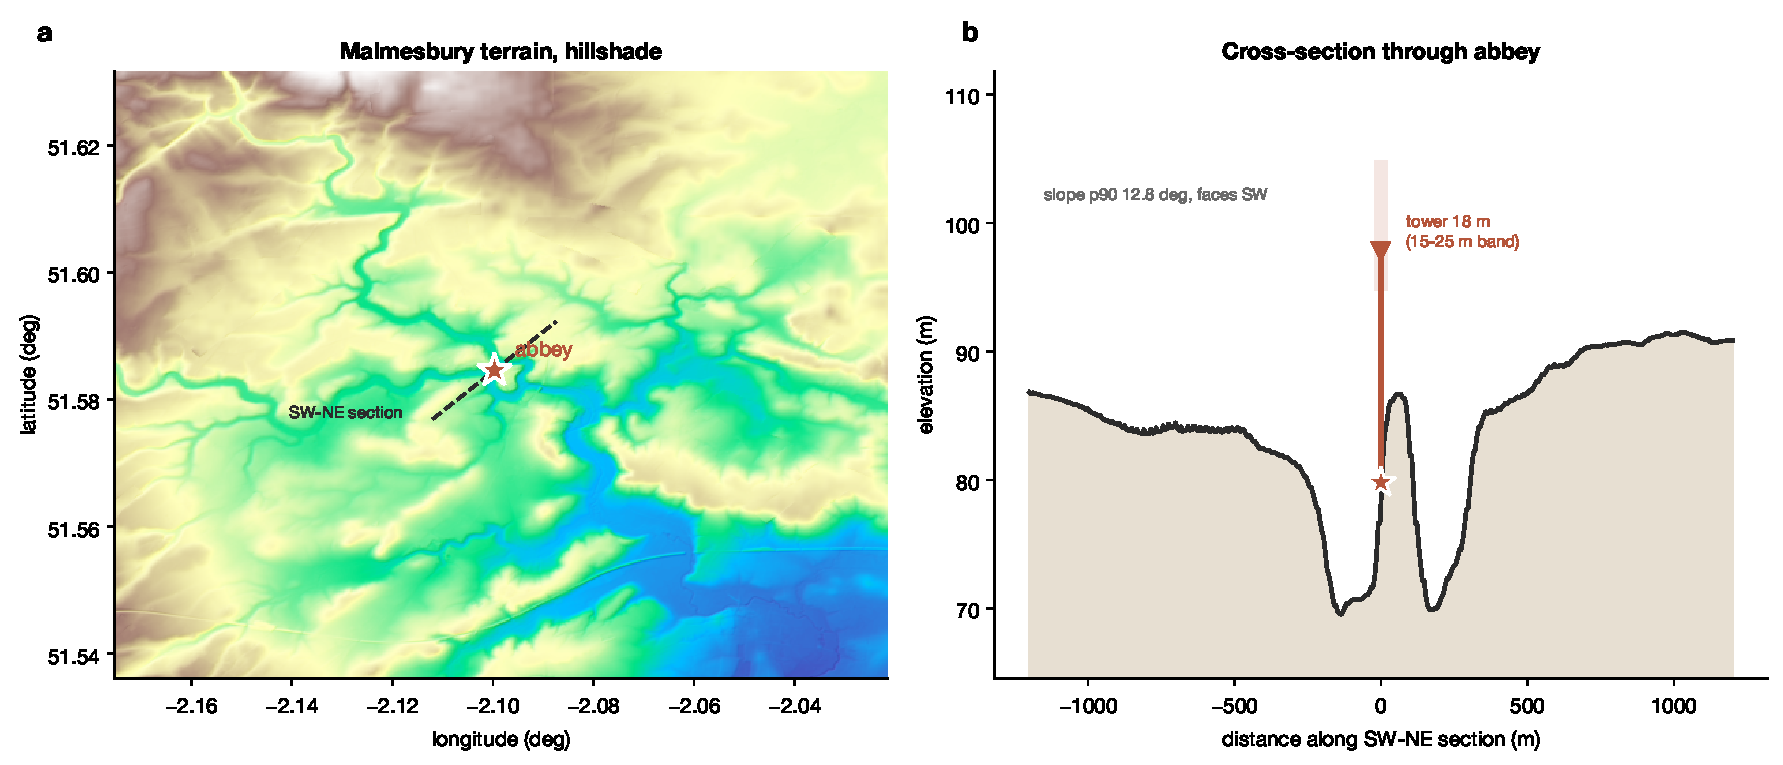
\includegraphics[width=\linewidth]{fig1_site}
  \caption{\textbf{Terrain at Malmesbury Abbey.}
  \textbf{(a)} Hillshaded DEM (AWS Terrain Tiles); the dashed line is the section in (c).
  \textbf{(b)} Southwest-facing ground steeper than \ang{\nSWFaceSlope} within \SI{\nSitePanel}{\meter} of the
  abbey (star), in orange.
  The green line is the track along the slope (\SI{\nLiftAlongSlope}{\meter}); the grey
  arrow is the first \SI{\nTarget}{\meter} of the track into the wind.
  \textbf{(c)} Elevation along the section, with the sampled tower heights.}
  \label{fig:site}
\end{figure}

\subsection{Wind climatology}

Hourly \SI{10}{\meter} wind at the abbey for 2004--2023 (\nHours\ hours) comes
from the ERA5 reanalysis of the European Centre for Medium-Range Weather Forecasts
\autocite{hersbach2020era5}, through the Open-Meteo archive
\autocite{openmeteo_archive}.
An hour is favourable when the wind blows from the southwest sector
(\ang{\nSectorLo}--\ang{\nSectorHi}, centred on the slope aspect) at \SIrange{\nSpeedLo}{\nSpeedHi}{\meter\per\second}.
Annual and seasonal fractions have \SI{95}{\percent} confidence intervals (CI) across the
twenty years.
Modern data stand in for the eleventh century.
Reconstructions of the North Atlantic Oscillation (NAO), the pressure pattern that sets the
strength of the westerlies over Britain, disagree on its medieval phase
\autocite{trouet2009nao,ortega2015nao}.
Neither indicates a long negative phase with weak westerlies.

\subsection{Ridge lift}

Wind blowing up a slope is deflected upwards, with a vertical velocity that to first order
follows the surface gradient and decays with height,
\begin{equation}
  w(x,z) = U\,\frac{\mathrm{d}h}{\mathrm{d}x}\,e^{-kz},
  \label{eq:ridge}
\end{equation}
where \(U\) is the wind speed, \(h(x)\) the terrain height along the wind, \(z\) the height
above the surface, and \(k = 2\pi/L\) with \(L\) the horizontal scale of the slope.
Supplementary \cref{fig:ridge} applies \cref{eq:ridge} to the measured section; the glide
model uses the simpler surface estimate \(w = \eta\,U\sin\theta_s\), where
\(\theta_s\) is the slope angle and \(\eta \le 1\) allows for flow that does not follow the
surface.
This lift extends \SI{\nLiftIntoWind}{\meter} on the track into the wind and
\SI{\nLiftAlongSlope}{\meter} on the track along the slope (\cref{fig:site}b).

\subsection{Glide performance}

The glide ratio \LD\ of an unknown wing follows from the parabolic drag polar
\(C_D = C_{D0} + C_L^2/(\pi e A)\), whose maximum is
\begin{equation}
  (\LD)_\mathrm{max} = \frac{1}{2}\sqrt{\frac{\pi e A}{C_{D0}}},
  \label{eq:polar}
\end{equation}
where \(A\) is the aspect ratio (span squared over area), \(e\) the span efficiency, and
\(C_{D0}\) the zero-lift drag coefficient \autocite{drela2014flight}.
An aspect ratio of \numrange{\nARlo}{\nARhi} gives a span of one to two arm spans for areas
of \SIrange{\nAreaLo}{\nAreaHi}{\meter\squared}.
Span efficiencies of \numrange{\nElo}{\nEhi} cover untwisted, non-elliptical wings
\autocite{drela2014flight}.
The zero-lift drag \(C_{D0} = \numrange{\nCDzlo}{\nCDzhi}\) adds the profile drag of a
cambered membrane at a Reynolds number near \num{e\nReExp}
\autocite{lissaman1983lowre,hoerner1985lift} to the drag of the pilot's body, frame and
bracing \autocite{hoerner1965drag}.
These ranges give \((\LD)_\mathrm{max} = \numrange{\nLDlo}{\nLDhi}\), with \num{\nLDnom}
at their centres.
Every wing is flown at its best glide ratio, which favours the account.

A wing of area \(S\) carrying mass \(m\) at lift coefficient \(C_L\) trims at
\(V = \sqrt{2mg/(\rho S C_L)}\), \SI{\nTrimSpeed}{\meter\per\second} for the nominal
configuration of \cref{fig:apparatus} (\SI{\nMass}{\kilogram}, \SI{\nArea}{\meter\squared},
\(C_L = \nCLtrim\)).

\begin{figure}[htbp]
  \centering
  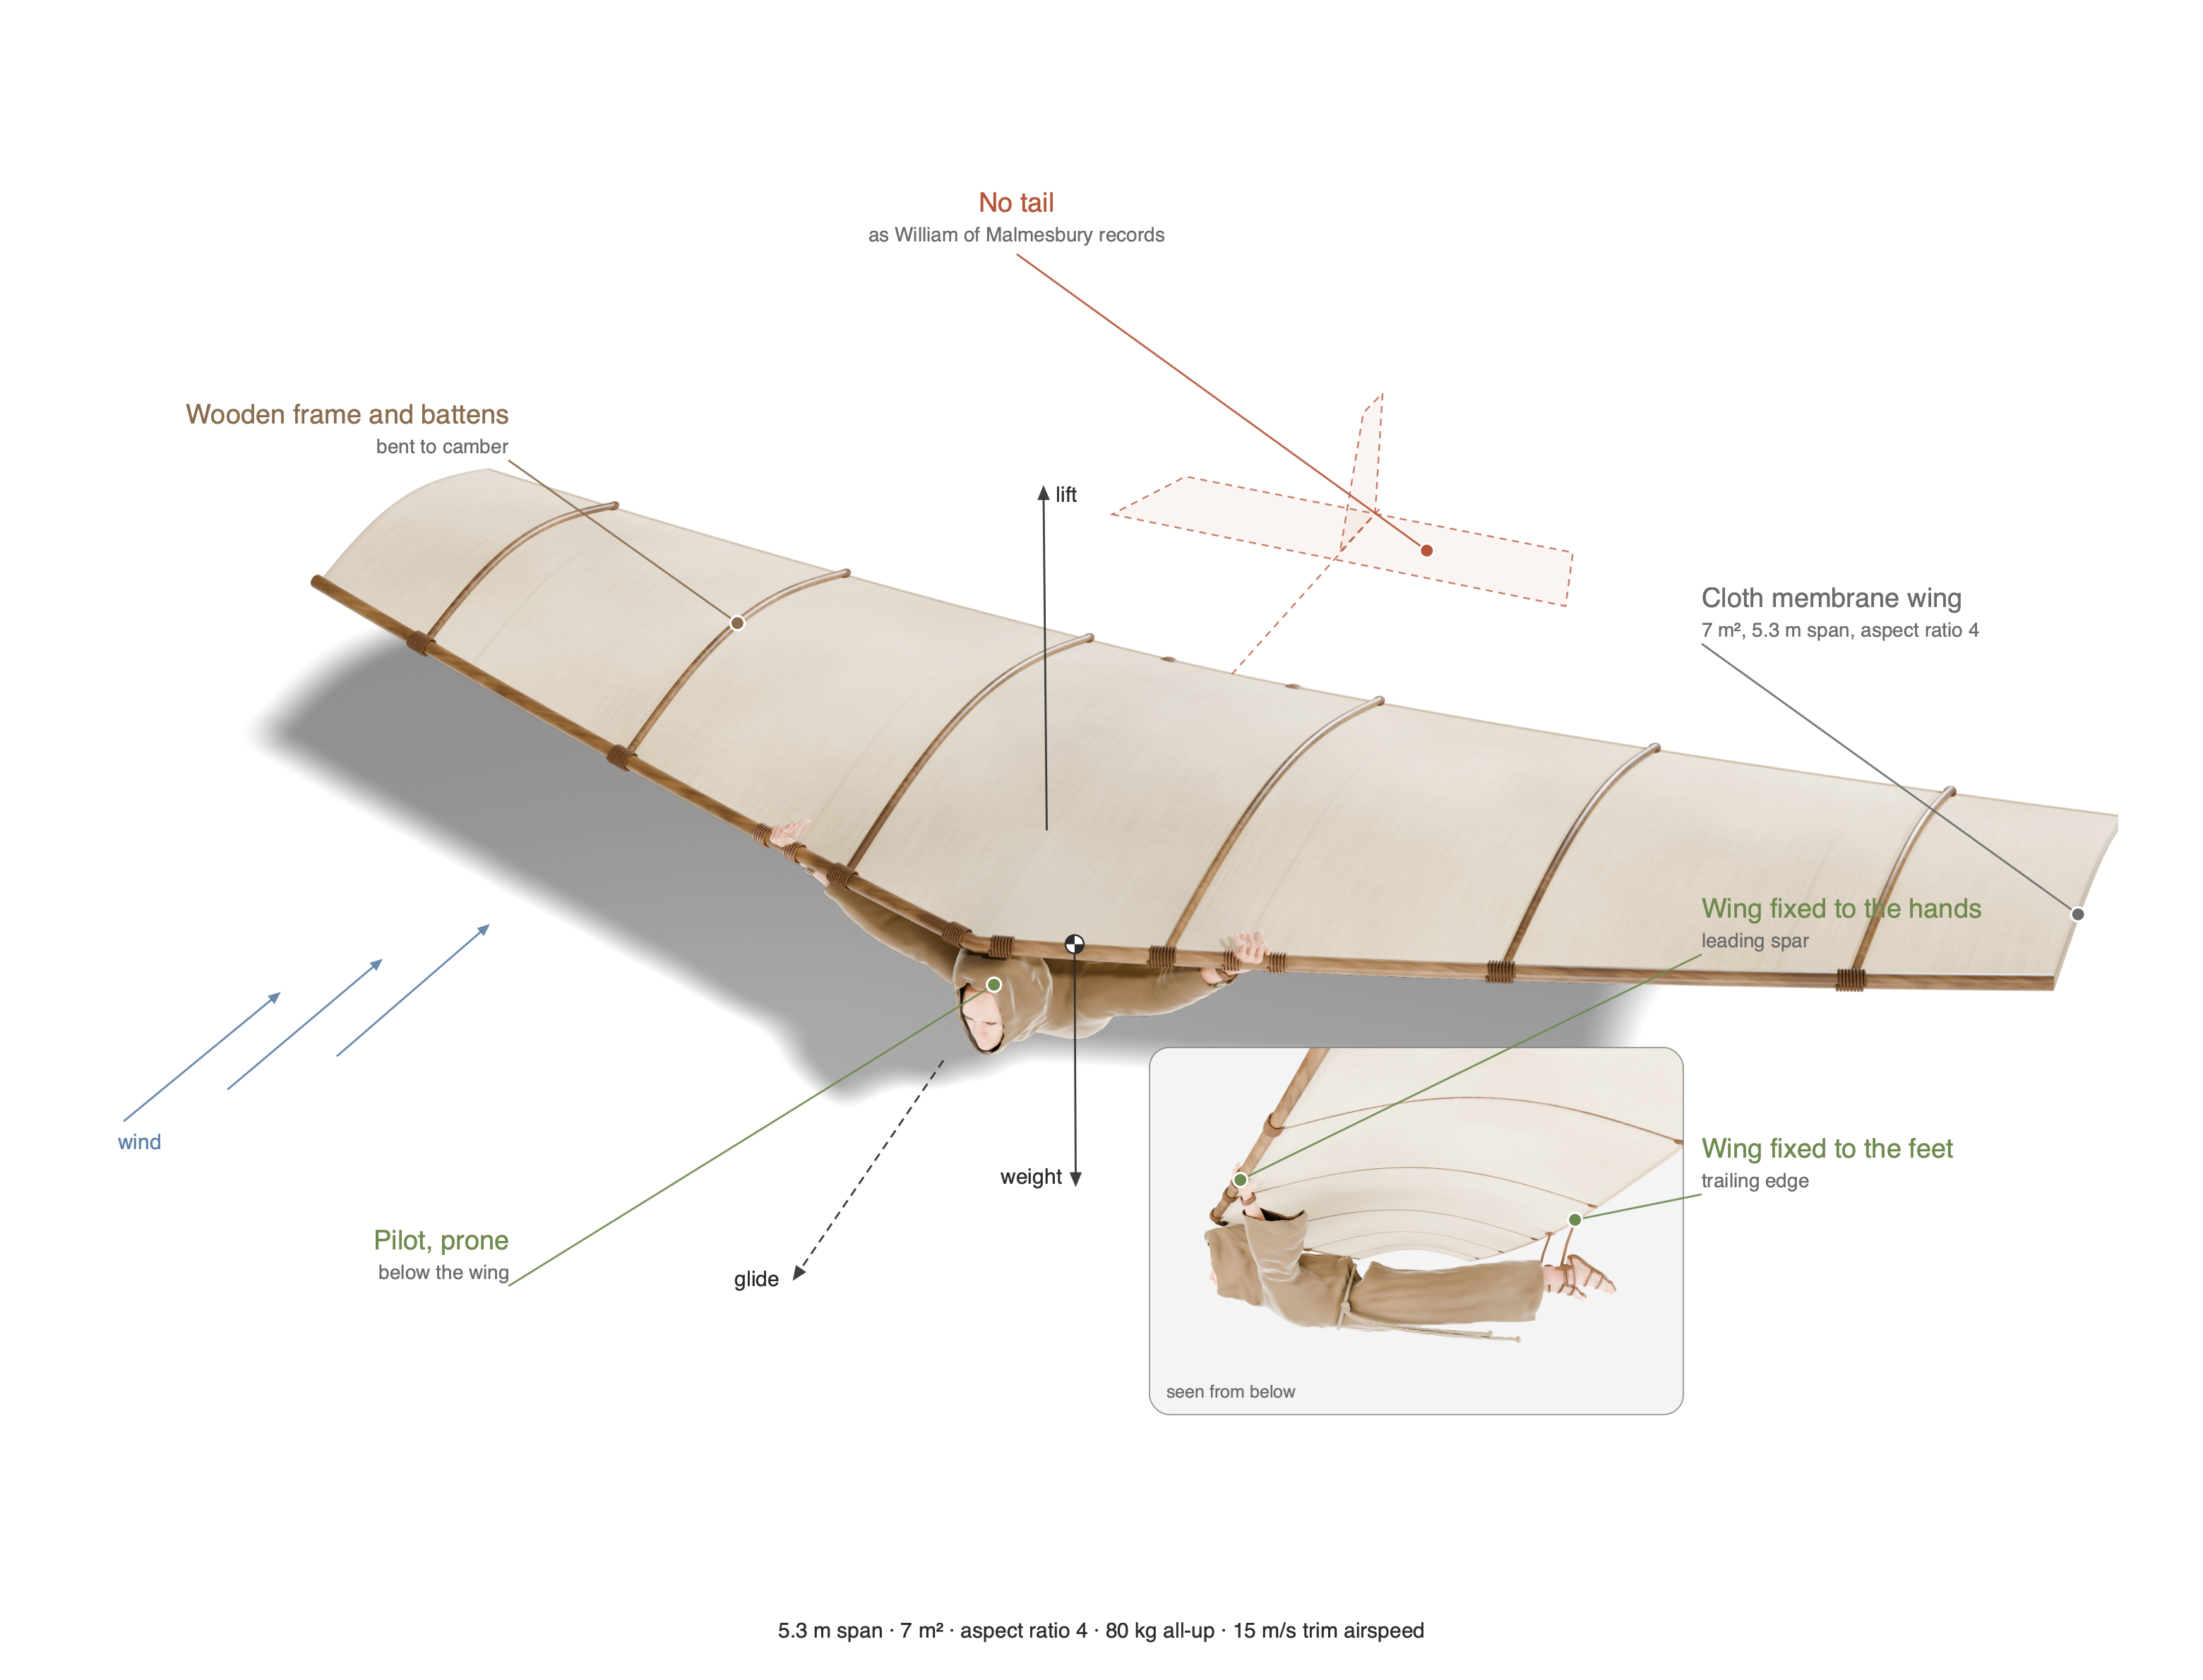
\includegraphics[width=0.75\linewidth]{fig_apparatus}
  \caption{\textbf{Nominal model configuration, not a reconstruction.}
  A tailless cloth wing fixed to the prone pilot's hands (leading edge) and feet (trailing
  edge).
  Only the attachment and the missing tail come from the source; the dimensions are the centres of the sampled
  ranges (Supplementary \cref{tab:priors}).
  The dashed outline marks where a tail would be; arrows show lift, weight, glide and headwind.}
  \label{fig:apparatus}
\end{figure}

\subsection{Launch and glide trajectory}

A man stepping off a tower leaves at about \SI{\nJump}{\meter\per\second} relative to the
ground and dives until the airspeed reaches \(V\), so the flight is integrated as a point mass at constant
\(C_L\),
\begin{equation}
  \dot V = g\sin\gamma - \frac{D}{m}, \qquad
  \dot\gamma = \frac{1}{V}\left(g\cos\gamma - \frac{L}{m}\right), \qquad
  \dot z = -V\sin\gamma + w,
  \label{eq:eom}
\end{equation}
where \(V\) is now the airspeed, \(\gamma\) the descent angle below the horizontal,
\(L = \frac{1}{2}\rho V^2 S C_L\), and \(D = L/(\LD)\).
The airspeed at release is the jump speed plus the headwind.

Two tracks bracket the ground covered.
On the first, the pilot heads southwest into the wind, down the slope towards the river
\autocite{woosnam1986eilmer}, at ground speed \(V\cos\gamma - U\) over the measured section.
On the second, he flies northwest along the slope with the wind from the side, as
hang-glider and sailplane pilots use ridge lift \autocite{faa_glider}.
He crabs, heading partly into the wind to hold the track, at ground speed
\(\sqrt{(V\cos\gamma)^2 - U^2}\) over a contour \SI{\nContour}{\meter} below the abbey.
William's ``more than a furlong'' becomes a ground range of at least \SI{\nTarget}{\meter}.

\subsection{Pitch stability}

A wing is stable in pitch if the centre of gravity (CG) lies ahead of the
neutral point, about which the pitching moment does not change with angle of attack.
Both are measured from the leading edge as fractions of the mean chord \(c\), \(\cgfrac\)
and \(\npfrac\).
A cambered wing without a tail has \(\npfrac \approx \nNPnotail\); a tail moves it aft, to
\num{\nNPtail} for the nominal tail, and adds pitch damping \autocite{drela2014flight}.

The pilot's mass centre lies between his hands, at the leading edge, and feet, at the
trailing edge.
Standing, it is at about \SI{\nComHeightPct}{\percent} of his height above the soles
\autocite{winter2009biomechanics}, and his reach from soles to raised hands is about
\num{\nReachRatio} times his height.
Laid out, it lies about \num{\nCGstraight} of the hand-to-foot distance behind the hands.
The sampled range \(\cgfrac = \numrange{\nCGlo}{\nCGhi}\) runs from this straight posture
forward to hips drawn up under the leading edge.
A wider sweep, \(\cgfrac = \numrange{\nCGsweepLo}{\nCGsweepHi}\), shows where the conclusion would change.

With the CG aft of the neutral point, the short-period motion, linearised in angle of attack
and pitch rate \autocite{drela2014flight}, has a positive real eigenvalue \(\lambda\), so a
disturbance doubles in \(t_2 = \ln 2/\lambda\).
\(t_2\) is compared with the flight time and a human operator's effective
time delay in manual control, about \SIrange{\nReactLo}{\nReactHi}{\second}
\autocite{mcruer1967pilot}.
A nonlinear run tests an \ang{\nGust} gust, with control lost beyond \ang{\nPitchLoss} of pitch.

\subsection{Monte Carlo sample}

Because the apparatus and the day are unknown, \nSamples\ cases are drawn with a fixed
seed from the uniform ranges of every parameter above (Supplementary
\cref{tab:priors}), except the glide ratio, which follows from \cref{eq:polar}.
The launch wind is drawn from the ERA5 southwest-sector hours at
\SIrange{\nWindLo}{\nWindHi}{\meter\per\second}, assuming Eilmer chose a windy day.
Each case is flown on both tracks with \cref{eq:eom} and scored on whether it covers
\SI{\nTarget}{\meter} and whether \(t_2\) is shorter than the flight, with and without a tail.
Fractions have Wilson score \SI{95}{\percent} CIs.

\subsection{Impact}

William records that Eilmer broke both legs and survived.
In a feet-first landing the body stops over a distance \(d\) of leg flexion and ground
give, so a vertical arrival speed \(v\) gives a mean force
\begin{equation}
  F = \frac{m v^2}{2 d}, \qquad \text{shared between two legs.}
  \label{eq:impact}
\end{equation}
The tibia breaks under axial and combined loads of \SIrange{\nTibiaLo}{\nTibiaHi}{\kilo\newton}
per leg \autocite{salzar2014leg,abidin2026tibia,forman2012femur,ivarsson2005bending,femurFE2022},
which sets a fracture-onset speed \(v^\star = \sqrt{2 d F_\mathrm{tot}/m}\) for
\(d = \SIrange{\nStopLo}{\nStopHi}{\centi\meter}\).
Two arrivals are compared for cases that reach \SI{\nTarget}{\meter}.
A controlled glide without a flare meets the ground at the vertical speed from
\cref{eq:eom}.
After a loss of pitch control the craft strikes at airspeed \(V\) along a path
\ang{\nDepAngLo}--\ang{\nDepAngHi} below horizontal, with vertical speed \(V\sin\theta\).
Because \cref{eq:impact} uses the mean force, peak loads are higher and the onset speeds are
upper bounds.

\section{Results}
\label{sec:results}

\subsection{Site and wind}

The abbey stands \SI{\nRelief}{\meter} above the valley floor on a spur whose flanks face
southwest (aspect \ang{\nAspect}), with a mean slope of \ang{\nSlopeMean} and a
90th-percentile slope of \ang{\nSlopePninety} within \SI{\nSlopeRadius}{\meter}
(\cref{fig:site}).
The southwest-facing ground near the abbey forms a strip \SI{\nLiftAlongSlope}{\meter} long
running northwest from the abbey; heading southwest, the ground reaches the valley floor
within \SI{\nLiftIntoWind}{\meter}.

Over twenty years the wind blows from the southwest sector at
\SIrange{5}{12}{\meter\per\second} in \SI{\nFavPct}{\percent} of hours
(\SI{95}{\percent} CI \SIrange{\nFavLo}{\nFavHi}{\percent}), about \nFavHours\ hours a year,
and in \SI{\nFavWinter}{\percent} of winter hours (\cref{fig:wind}).
Strong southwest winds are rarer: \SI{6}{\meter\per\second} or more in
\SI{\nSWSixPct}{\percent} of hours (\nSWSixHours\ hours a year), and
\SI{8}{\meter\per\second} or more in \SI{\nSWEightPct}{\percent}
(CI \SIrange{\nSWEightLo}{\nSWEightHi}{\percent}; \nSWEightHours\ hours a year).

\begin{figure}[htbp]
  \centering
  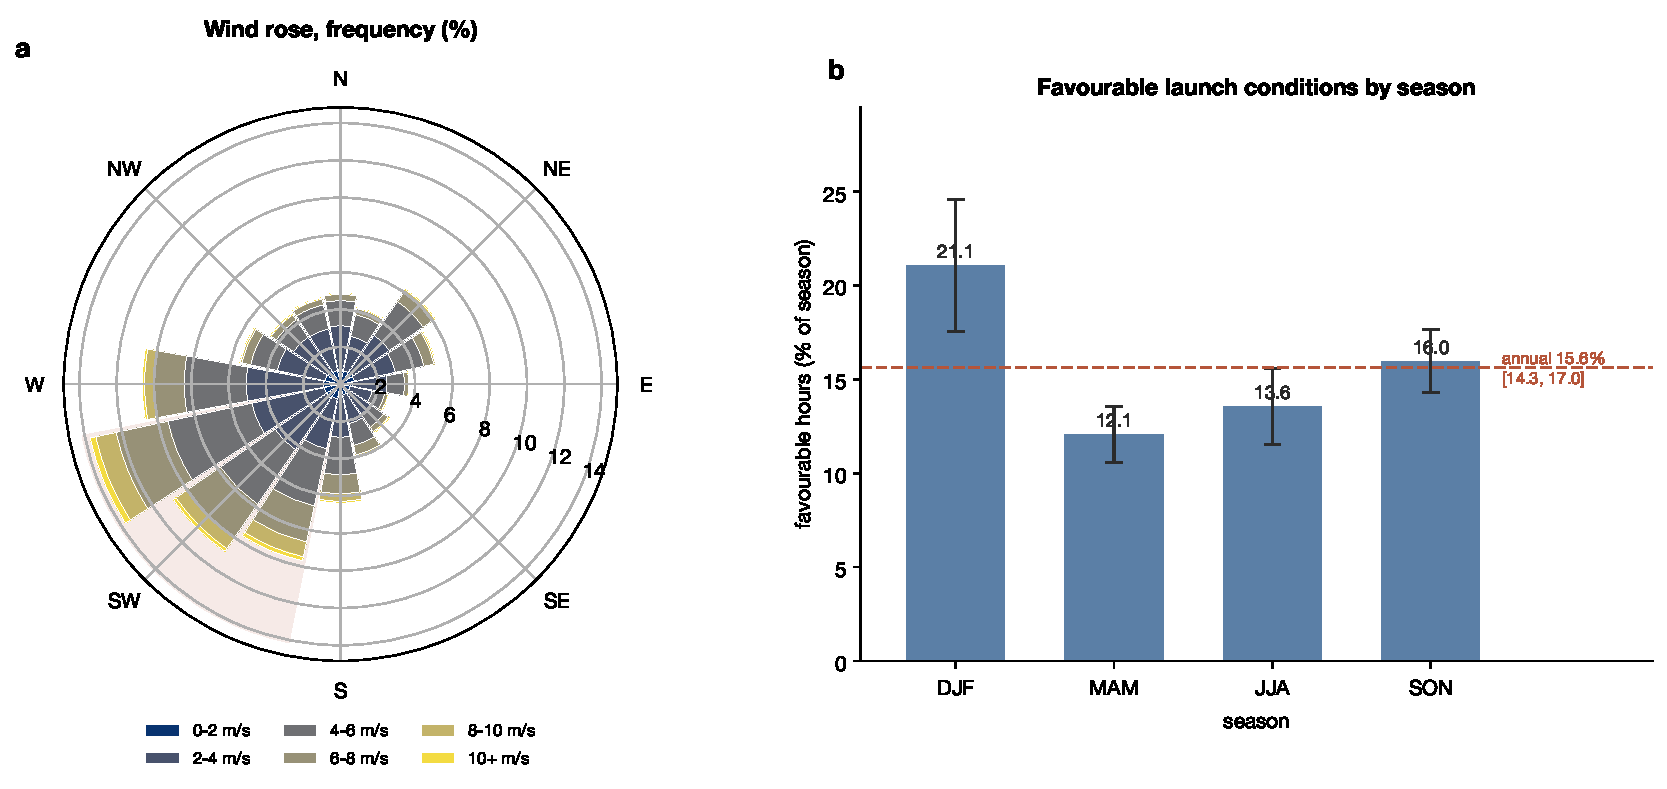
\includegraphics[width=\linewidth]{fig2_wind}
  \caption{\textbf{Wind at the abbey, 2004--2023.}
  \textbf{(a)} Wind rose of ERA5 hourly \SI{10}{\meter} wind (\nHours\ hours).
  \textbf{(b)} Fraction of hours from the southwest sector (\ang{191}--\ang{259}) at
  \SIrange{5}{12}{\meter\per\second}, for the year and by season (DJF, December--February;
  MAM, March--May; JJA, June--August; SON, September--November), with \SI{95}{\percent}
  confidence intervals across the twenty years.}
  \label{fig:wind}
\end{figure}

The linear model (\cref{eq:ridge}) gives a peak upward air speed of
\SI{\nRidgePeak}{\meter\per\second} just southwest of the abbey in an
\SI{\nRidgeWind}{\meter\per\second} wind (Supplementary \cref{fig:ridge}), close to the
surface estimate \(U\sin\theta_s = \SI{\nRidgeFormula}{\meter\per\second}\) at the
90th-percentile slope.
The still-air sink rate of the nominal craft at its best glide is
\(V/\sqrt{1+(\LD)^2}\): \SI{\nSinkBest}{\meter\per\second} at \LD~\num{\nLDhi} and
\SI{\nSinkNominal}{\meter\per\second} at \LD~\num{\nLDnom}.
Ridge lift can therefore roughly cancel the sink of the better wings in a strong wind, and
not that of the poorer ones.

\subsection{Launch and glide}

In still air, a steady glide from the \SI{\nTower}{\meter} tower would cover
\SI{200}{\meter} only with \LD~\num{\nLDStillSteady}, beyond the range of
\cref{eq:polar}.
A standing launch does much worse.
Reaching \SI{\nTrimSpeed}{\meter\per\second} from \SI{\nJump}{\meter\per\second} costs
\((V^2 - v_0^2)/2g \approx \SI{\nHeightToTrim}{\meter}\) of height, and the best wing,
\LD~\num{\nLDhi}, lands \SI{\nStillRangeBest}{\meter} from the tower instead of the
\SI{\nStillRangeSteady}{\meter} of a steady glide (\cref{fig:glide}b).
A headwind supplies airspeed at release without the dive, which is why the wind matters for
the launch as well as for the lift.

Into the wind, the headwind that eases the launch also slows the craft over the ground,
and the lift ends within \SI{\nLiftIntoWind}{\meter}.
None of the three wings in \cref{fig:glide}a reaches \SI{200}{\meter} on this track at any
wind up to \SI{14}{\meter\per\second}; the longest flight is \SI{\nMaxRangeInto}{\meter}
(dashed lines).
Along the slope, the lift lasts for \SI{\nLiftAlongSlope}{\meter}, and a crabbing craft can
stay in it.
The best wing reaches \SI{200}{\meter} from a \SI{\nTower}{\meter} tower above
\SI{\nMinWindBest}{\meter\per\second} of wind and the central wing above
\SI{\nMinWindNominal}{\meter\per\second}; the poorest wing does not reach it at any wind
(\cref{fig:glide}a, solid).
The threshold for the best wing moves from \SI{\nMinWindTowerHi}{\meter\per\second} to
\SI{\nMinWindTowerLo}{\meter\per\second} as the tower height falls from \SI{25}{\meter} to
\SI{15}{\meter}.

\begin{figure}[htbp]
  \centering
  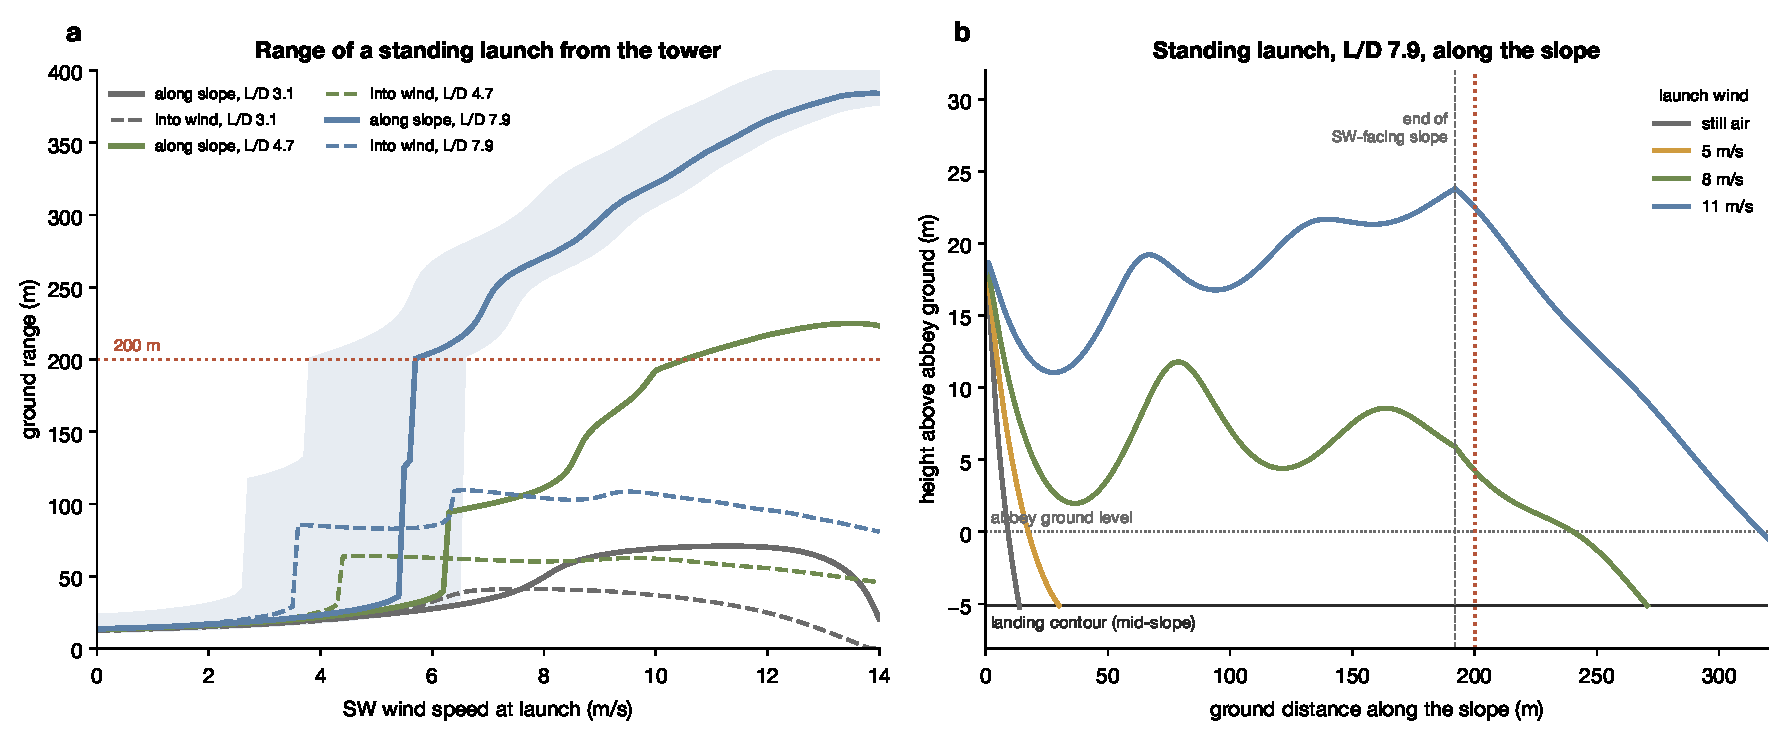
\includegraphics[width=\linewidth]{fig4_glide_envelope}
  \caption{\textbf{Range of a standing launch from the tower.}
  \textbf{(a)} Ground range against launch wind for the nominal craft (\cref{fig:apparatus})
  launched from \SI{\nTower}{\meter} at \SI{\nJump}{\meter\per\second}, for the lowest,
  central, and highest glide ratios of the drag-polar range, on the track along the slope
  (solid) and into the wind (dashed).
  The shaded band is the best wing along the slope for towers of \SIrange{15}{25}{\meter}.
  The step near \SI{5.5}{\meter\per\second} is where ridge lift first matches the sink of
  the best wing.
  \textbf{(b)} Trajectories along the slope for the best wing (\LD~\num{\nLDhi}).
  In still air the craft dives to gain speed and lands \SI{\nStillRangeBest}{\meter} out; in
  wind it climbs and falls in the lift and descends once past the end of the
  southwest-facing slope.}
  \label{fig:glide}
\end{figure}

\subsection{Pitch stability}

Without a tail the neutral point is at \num{\nNPnotail}\,\(c\), ahead of every sampled CG,
so the wing is statically unstable in pitch (\cref{fig:stability}).
Pitch damping delays the divergence until the CG is aft of \num{\nCGonset}\,\(c\).
Across the sampled CG range the doubling time falls from \SI{\nTdoubleFwd}{\second} at
\num{\nCGlo}\,\(c\) to \SI{\nTdoubleAft}{\second} at \num{\nCGhi}\,\(c\)
(\SIrange{\nTdoubleInLo}{\nTdoubleInHi}{\second} when the pitch inertia is halved or
doubled); a \SI{200}{\meter} flight of the nominal craft lasts about
\SI{\nFlightTime}{\second}.
After an \ang{8} gust the tailless craft passes \ang{60} of pitch in
\SI{\nTloss}{\second}.
With a tail the same gust dies away.

\begin{figure}[htbp]
  \centering
  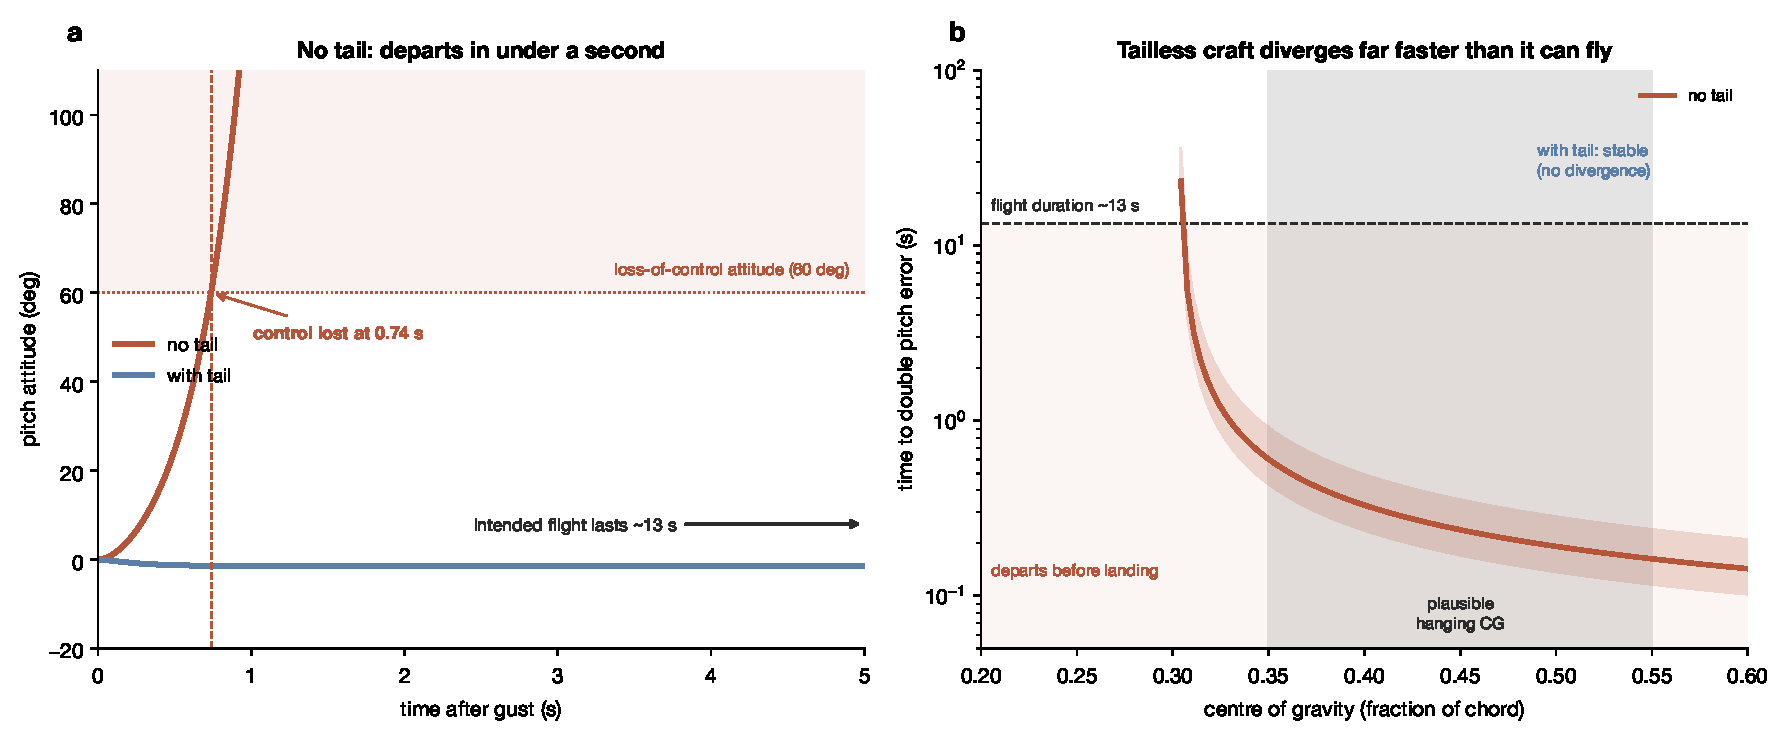
\includegraphics[width=\linewidth]{fig5_stability}
  \caption{\textbf{Pitch stability with and without a tail.}
  \textbf{(a)} Pitch attitude after an \ang{8} gust for the nominal craft with its CG at
  mid-range.
  Without a tail the attitude passes \ang{60} after \SI{\nTloss}{\second}; with a tail the
  disturbance damps out.
  \textbf{(b)} Time for a pitch disturbance to double against CG position for the tailless
  craft; the band is pitch inertia from half to twice nominal.
  The grey band is the sampled CG range and the tan band the effective time delay of a human
  operator \autocite{mcruer1967pilot}.
  The tailed craft does not diverge at any CG shown.}
  \label{fig:stability}
\end{figure}

\subsection{Monte Carlo sample}

Into the wind, none of the \nSamples\ cases reaches \SI{200}{\meter}
(\SI{95}{\percent} upper bound \SI{\nReachIntoHi}{\percent}); the median range is
\SI{\nMedRangeInto}{\meter} (\cref{fig:montecarlo}a).
Along the slope, \nReachSlopeN\ cases do, \SI{\nReachSlope}{\percent}
(CI \SIrange{\nReachSlopeLo}{\nReachSlopeHi}{\percent}), against a median range of
\SI{\nMedRangeSlope}{\meter} and a 90th percentile of \SI{\nNinetyRangeSlope}{\meter}.
The cases that reach it share a strong wind and a good wing: their median launch wind is
\SI{\nMedWindReach}{\meter\per\second} (\SI{90}{\percent} above
\SI{\nTenWindReach}{\meter\per\second}), and their median glide ratio is \num{\nMedLDReach},
against \num{\nMedLDAll} over all cases.
\SI{\nShortFifty}{\percent} of all cases land within \SI{50}{\meter} of the tower.

Among the cases that reach \SI{200}{\meter}, the tailless doubling time has a median of
\SI{\nTdoubleMC}{\second} (99th percentile \SI{\nTdoubleMCpnn}{\second}) and the flight a
median of \SI{\nMedFlightReach}{\second} (\cref{fig:montecarlo}b).
In every one of them the doubling time is shorter than the flight, and with a tail none
diverges.

\begin{figure}[htbp]
  \centering
  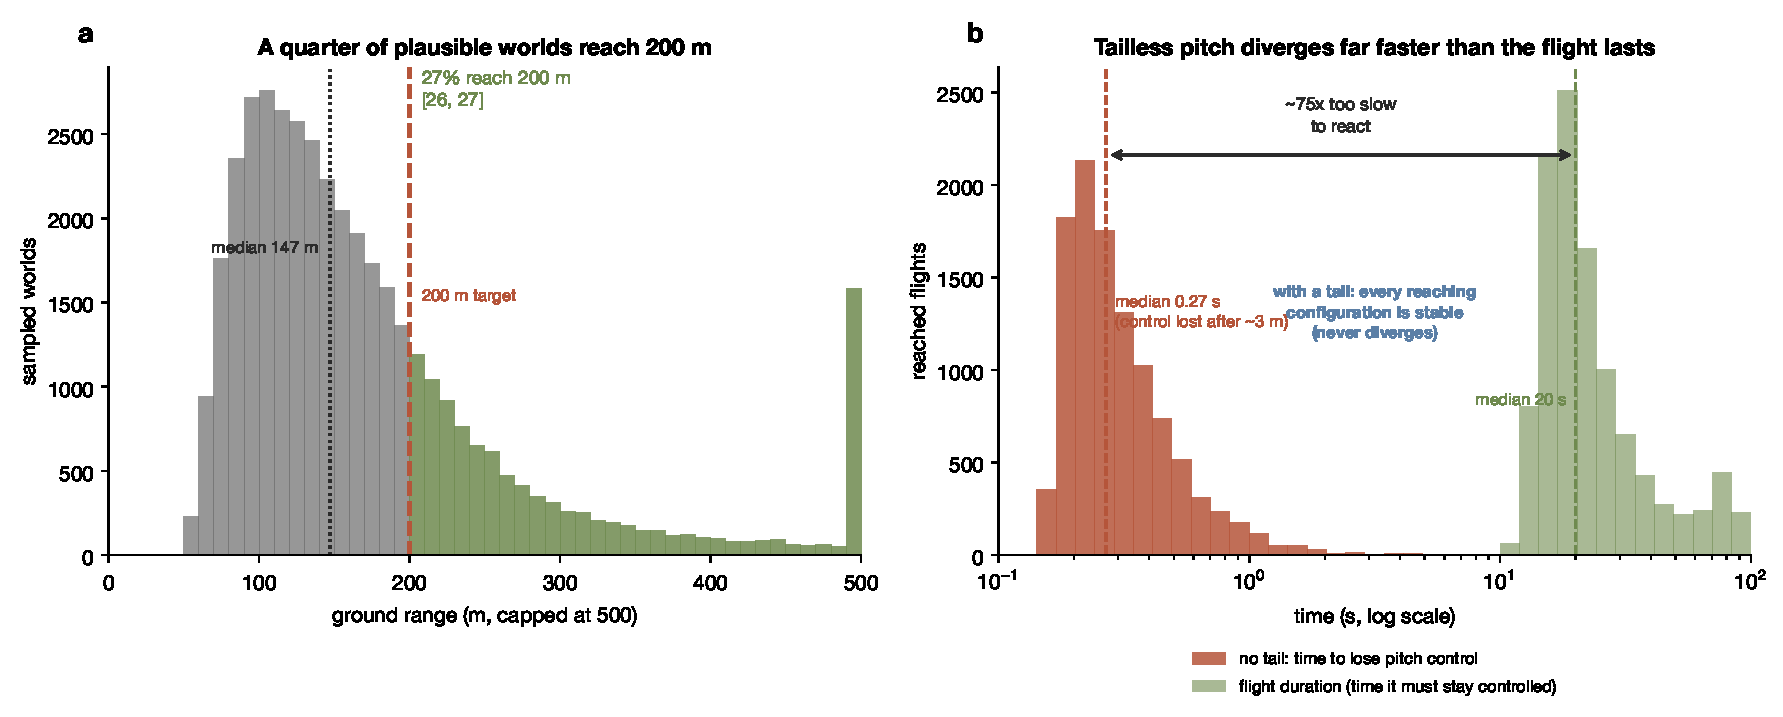
\includegraphics[width=\linewidth]{fig6_montecarlo}
  \caption{\textbf{Monte Carlo sample of \nSamples\ apparatus and launch-day cases.}
  Parameters are drawn from Supplementary \cref{tab:priors}, and the launch wind from the
  ERA5 southwest-sector hours.
  \textbf{(a)} Ground range on the two tracks.
  Along the slope \SI{\nReachSlope}{\percent} of cases reach \SI{200}{\meter}
  (\SI{95}{\percent} CI \SIrange{\nReachSlopeLo}{\nReachSlopeHi}{\percent}); into the wind
  none does.
  \textbf{(b)} For the \nReachSlopeN\ cases that reach \SI{200}{\meter} along the slope, the
  time for a pitch disturbance to double without a tail, and the duration of the flight.
  The tan band is the effective time delay of a human operator.}
  \label{fig:montecarlo}
\end{figure}

\subsection{Impact}

For \(d = \SI{20}{\centi\meter}\) the legs break above about
\SI{\nOnsetMid}{\meter\per\second} of vertical speed, and the onset ranges from
\SI{\nOnsetLo}{\meter\per\second} to \SI{\nOnsetHi}{\meter\per\second} across the stopping
distances and fracture loads (\cref{fig:biomech}a).
A controlled glide that ends without a flare meets the ground at a median
\SI{\nCtrlVzMed}{\meter\per\second} and at most \SI{\nCtrlVzMax}{\meter\per\second} of
vertical speed, below the lowest onset speed, so it does not break the legs even without a
flare (\cref{fig:biomech}b).
An arrival after loss of pitch control, at airspeeds of
\SIrange{\nVreachLo}{\nVreachHi}{\meter\per\second}, has a median vertical speed of
\SI{\nDepVzMed}{\meter\per\second}; \SI{\nPbreakDep}{\percent} of such arrivals exceed the
central onset speed.
The median deceleration over \SI{20}{\centi\meter} is about \num{\nDecelG}\,\(g\), which
feet-first falls are commonly survived.

\begin{figure}[htbp]
  \centering
  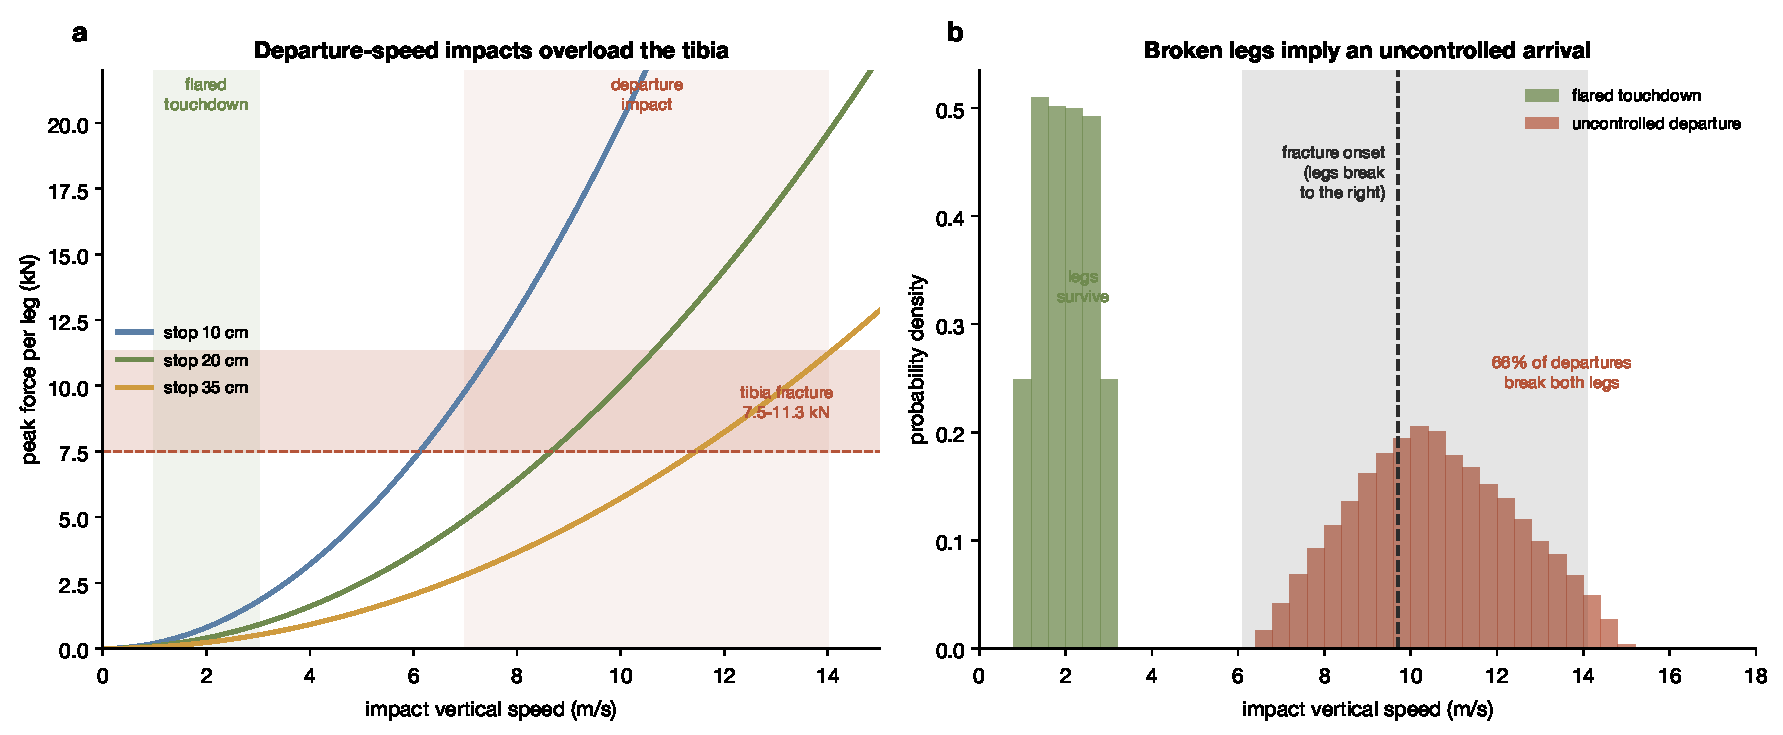
\includegraphics[width=\linewidth]{fig7_biomech}
  \caption{\textbf{Arrival speed and leg fracture.}
  \textbf{(a)} Mean feet-first impact force per leg against vertical speed for stopping
  distances of \SIrange{10}{35}{\centi\meter}, with the tibia fracture range
  (\SIrange{\nTibiaLo}{\nTibiaHi}{\kilo\newton} per leg).
  \textbf{(b)} Vertical arrival speeds of the \nReachSlopeN\ cases that reach
  \SI{200}{\meter}, for a controlled glide that ends without a flare and for an arrival
  after loss of pitch control (\(V\sin\theta\), \(\theta =
  \ang{\nDepAngLo}\text{--}\ang{\nDepAngHi}\)).
  The grey band is the range of fracture-onset speeds and the dashed line its centre.}
  \label{fig:biomech}
\end{figure}
\FloatBarrier

\section{Discussion}
\label{sec:discussion}

\subsection{What the account requires}

Read against the models, William's account describes a narrow set of conditions.
A flight of a furlong from a tower of this height needs a strong southwest wind, a wing
near the better end of what cloth and timber allow, and a track that stays over the
slope.
Flying straight out over the valley, the route \textcite{woosnam1986eilmer} proposed, does
not reach \SI{200}{\meter} in any sampled case, because the headwind slows the craft over
the ground and the lift ends at the foot of the slope.
Flying along the slope reaches it in \SI{\nReachSlope}{\percent} of cases.
Southwest winds of \SI{8}{\meter\per\second} or more blow for about \nSWEightHours\ hours a
year, so a man who waited for one would not have waited long.
William's phrase that Eilmer ``collected the breeze'' fits a launch timed to such a wind.

Without a tail the craft diverges in pitch in a fraction of a second, but the doubling time
is close to human reaction time rather than far below it.
A pilot who moves his body could therefore hold the attitude for a while by continual
correction, and a flight of tens of seconds followed by a loss of control is consistent
with the model.
The account names the trigger: the violence of the wind and the swirling of the air.
A gust large enough to need a correction faster than his reactions would end the flight in
under a second (\cref{fig:stability}a).
The models do not show that he lost control, only that he would have been unlikely to keep
it and that a tail would have removed the need to.

The broken legs are consistent with a loss of control but do not prove one.
A controlled glide into the ground without a flare arrives too slowly to break the legs in
this model, so the injury requires a fast, steep arrival.
A loss of pitch control gives that, but so would a stall at height or a dive into the
ground that is not caused by the missing tail.

\subsection{Which results depend on the assumptions}

Three results follow from measurement or from simple bounds and would survive large
changes to the model.
The slope faces the prevailing wind, and strong southwest winds are measured to occur
(\cref{fig:site,fig:wind}).
The launch dive costs \((V^2-v_0^2)/2g\) of height whatever the wing, so a still-air flight
of a furlong is not possible from this tower.
A tailless wing is unstable in pitch whenever the CG is aft of about \num{\nCGonset}\,\(c\),
and for a man fixed to the wing at his hands and feet the CG is near mid-chord.
This last result holds if the sampled CG range brackets the real posture;
\cref{fig:stability}b shows it would fail only if the pilot's mass centre lay ahead of
\num{\nCGonset}\,\(c\), within the front of the chord near his hands.

The fraction of cases reaching \SI{200}{\meter} depends on the ranges in Supplementary
\cref{tab:priors}, and should be read as the share of the sampled ranges that works, not as
a probability that the flight happened.
It is most sensitive to the glide ratio and the strength and length of the ridge lift.
The glide ratio rests on \cref{eq:polar} with bounds on aspect ratio, span efficiency, and
drag, and every wing is flown at its best glide, which favours the account.
The lift rests on a first-order model over a smoothed \SI{6}{\meter} terrain grid; the real
slope is steeper than the grid shows, which would raise the lift, while turbulence and
separation behind the spur edge would lower it.
The point-mass model holds \(C_L\) fixed, so it does not let the pilot trade height for speed
more efficiently than a stable glider would, and the pitch analysis treats the longitudinal
motion alone.
A large-eddy simulation over LIDAR terrain and a six-degree-of-freedom model with a pilot
model would narrow these margins.

\subsection{Limits of the comparison}

The comparison with the text assumes that a furlong means about \SI{200}{\meter} of ground,
that the tower stood at or near the abbey, and that William reports what Eilmer said.
A shorter flight would be easier to explain; a tower on lower ground would be harder.
None of the models tests whether the structure could carry the flight loads, which would be
a separate failure mode.

\section{Using the study in teaching}
\label{sec:teaching}

The analysis divides into exercises that each use one topic from a first or second year
mechanics course and one public data set or short script.
They can be set singly, as problems, or together as a project in which students rebuild a
figure and then change one assumption.
Worked answers are in Supplementary S4.

\begin{enumerate}
  \item \textbf{Energy at launch.}
  A glider leaves a tower of height \(H\) at \(v_0 = \SI{\nJump}{\meter\per\second}\) and needs
  \(V = \SI{\nTrimSpeed}{\meter\per\second}\) to fly.
  Ignoring drag, find the height lost in reaching \(V\).
  How large a headwind makes the launch dive unnecessary?
  Integrate \cref{eq:eom} numerically in still air and compare the range with the steady
  glide estimate \(H\,(\LD)\).

  \item \textbf{Glide ratio from a drag polar.}
  Derive \cref{eq:polar} by minimising \(C_D/C_L\).
  Evaluate it at the corners of the ranges in Supplementary \cref{tab:priors}.
  Which parameter does the glide ratio depend on most, and which measurement on a model
  wing would narrow it?

  \item \textbf{Flight in a moving air mass.}
  Draw the velocity triangle for a craft of airspeed \(V\) heading into a wind \(U\), and for
  one crabbing along a track perpendicular to it.
  Show that the ground speeds are \(V - U\) and \(\sqrt{V^2-U^2}\).
  Explain why a headwind helps the launch and shortens the range on the first track.

  \item \textbf{Ridge lift and sink.}
  The upward air speed over a slope of angle \(\theta_s\) is about \(U\sin\theta_s\).
  The still-air sink rate is \(V/\sqrt{1+(\LD)^2}\).
  Find the wind at which the two are equal for \LD~\num{\nLDnom} and \LD~\num{\nLDhi} on a
  slope of \ang{\nSlopePninety}, and compare the answers with the ERA5 wind distribution.

  \item \textbf{Static and dynamic pitch stability.}
  Write the two-state short-period model in angle of attack and pitch rate.
  Show that a positive real eigenvalue appears when the CG moves aft of a point that depends
  on the pitch damping, and compute the doubling time for the nominal craft at
  \(\cgfrac = 0.45\).
  Compare it with your own reaction time, measured with a ruler-drop test.

  \item \textbf{Monte Carlo estimation.}
  Rerun the Monte Carlo with a different seed and sample size.
  Compute the Wilson interval for \nReachSlopeN\ successes in \nSamples\ trials by hand.
  Change one range in \cref{tab:priors} and report how the reach fraction moves.

  \item \textbf{Impact.}
  From \cref{eq:impact}, find the vertical speed that breaks a tibia for stopping distances of
  \SIrange{10}{35}{\centi\meter}.
  Estimate the vertical speed of a craft flying at \(V\) along a path \ang{50} below horizontal,
  and of one that glides into the ground at its sink rate.
  What does each tell you about how Eilmer landed?
\end{enumerate}

Exercises 2 and 6 ask students to work with quantities nobody measured: to bound them from
physical arguments, sample them, and find which conclusions change when a bound moves.

\section{Conclusion}

A furlong's flight from the abbey tower is physically possible for a cloth wing, but only
in a strong southwest wind, with a wing near the better end of what the materials allow,
and on a track that follows the slope.
A flight straight out over the valley does not reach that distance in any sampled case.
Without a tail the craft is unstable in pitch, with a disturbance doubling in about the
time a man takes to react, so a flight of some tens of seconds followed by a loss of control
in a gust fits the models; a tail removes the instability.
The broken legs require a fast, steep arrival, which a loss of control provides.
Eilmer's own explanation of his fall is consistent with the physics, though the physics
cannot show that it was the only cause.

\section*{Data and code availability}

\ifdefined\anon
The analysis code, data manifests, and figure scripts reproduce every number and figure in
this paper.
They are openly available in a public repository archived with a DOI; the links are
withheld for double-anonymous review and have been supplied to the editors.
\else
The analysis code, data manifests, and figure scripts reproduce every number and figure in
this paper.
They are openly available, and archived with a DOI, at
\begin{center}
\url{https://github.com/silverdavi/eilmer-flight-feasibility}\\
\url{https://doi.org/10.5281/zenodo.20706321}
\end{center}

\section*{Acknowledgements}

The author thanks the Athelstan Museum, Malmesbury, for its local record of Eilmer's flight,
and Dr Duncan Pepper for the photograph in \cref{fig:photo}, published under a CC BY-SA 2.0
licence.
This research received no specific funding.
\fi


\printbibliography


\end{document}
